%File: anonymous-submission-latex-2024.tex
\documentclass[letterpaper]{article} % DO NOT CHANGE THIS
\usepackage[submission]{aaai24}  % DO NOT CHANGE THIS
\usepackage{times}  % DO NOT CHANGE THIS
\usepackage{helvet}  % DO NOT CHANGE THIS
\usepackage{courier}  % DO NOT CHANGE THIS
\usepackage[hyphens]{url}  % DO NOT CHANGE THIS
\usepackage{graphicx} % DO NOT CHANGE THIS
\urlstyle{rm} % DO NOT CHANGE THIS
\def\UrlFont{\rm}  % DO NOT CHANGE THIS
\usepackage{natbib}  % DO NOT CHANGE THIS AND DO NOT ADD ANY OPTIONS TO IT
\usepackage{caption} % DO NOT CHANGE THIS AND DO NOT ADD ANY OPTIONS TO IT
\frenchspacing  % DO NOT CHANGE THIS
\setlength{\pdfpagewidth}{8.5in} % DO NOT CHANGE THIS
\setlength{\pdfpageheight}{11in} % DO NOT CHANGE THIS
%
% These are recommended to typeset algorithms but not required. See the subsubsection on algorithms. Remove them if you don't have algorithms in your paper.
\usepackage{algorithm}
\usepackage{algorithmic}

%
% These are are recommended to typeset listings but not required. See the subsubsection on listing. Remove this block if you don't have listings in your paper.
\usepackage{newfloat}
\usepackage{listings}
\DeclareCaptionStyle{ruled}{labelfont=normalfont,labelsep=colon,strut=off} % DO NOT CHANGE THIS
\lstset{%
	basicstyle={\footnotesize\ttfamily},% footnotesize acceptable for monospace
	numbers=left,numberstyle=\footnotesize,xleftmargin=2em,% show line numbers, remove this entire line if you don't want the numbers.
	aboveskip=0pt,belowskip=0pt,%
	showstringspaces=false,tabsize=2,breaklines=true}
\floatstyle{ruled}
\newfloat{listing}{tb}{lst}{}
\floatname{listing}{Listing}
%
% Keep the \pdfinfo as shown here. There's no need
% for you to add the /Title and /Author tags.
\pdfinfo{
/TemplateVersion (2024.1)
}

% DISALLOWED PACKAGES
% \usepackage{authblk} -- This package is specifically forbidden
% \usepackage{balance} -- This package is specifically forbidden
% \usepackage{color (if used in text)
% \usepackage{CJK} -- This package is specifically forbidden
% \usepackage{float} -- This package is specifically forbidden
% \usepackage{flushend} -- This package is specifically forbidden
% \usepackage{fontenc} -- This package is specifically forbidden
% \usepackage{fullpage} -- This package is specifically forbidden
% \usepackage{geometry} -- This package is specifically forbidden
% \usepackage{grffile} -- This package is specifically forbidden
% \usepackage{hyperref} -- This package is specifically forbidden
% \usepackage{navigator} -- This package is specifically forbidden
% (or any other package that embeds links such as navigator or hyperref)
% \indentfirst} -- This package is specifically forbidden
% \layout} -- This package is specifically forbidden
% \multicol} -- This package is specifically forbidden
% \nameref} -- This package is specifically forbidden
% \usepackage{savetrees} -- This package is specifically forbidden
% \usepackage{setspace} -- This package is specifically forbidden
% \usepackage{stfloats} -- This package is specifically forbidden
% \usepackage{tabu} -- This package is specifically forbidden
% \usepackage{titlesec} -- This package is specifically forbidden
% \usepackage{tocbibind} -- This package is specifically forbidden
% \usepackage{ulem} -- This package is specifically forbidden
% \usepackage{wrapfig} -- This package is specifically forbidden
% DISALLOWED COMMANDS
% \nocopyright -- Your paper will not be published if you use this command
% \addtolength -- This command may not be used
% \balance -- This command may not be used
% \baselinestretch -- Your paper will not be published if you use this command
% \clearpage -- No page breaks of any kind may be used for the final version of your paper
% \columnsep -- This command may not be used
% \newpage -- No page breaks of any kind may be used for the final version of your paper
% \pagebreak -- No page breaks of any kind may be used for the final version of your paperr
% \pagestyle -- This command may not be used
% \tiny -- This is not an acceptable font size.
% \vspace{- -- No negative value may be used in proximity of a caption, figure, table, section, subsection, subsubsection, or reference
% \vskip{- -- No negative value may be used to alter spacing above or below a caption, figure, table, section, subsection, subsubsection, or reference

\setcounter{secnumdepth}{0} %May be changed to 1 or 2 if section numbers are desired.

\usepackage{amsmath}
\usepackage{amssymb}
\usepackage{amsthm}
\usepackage{todonotes}
\usepackage{bm}
\usepackage{subcaption}
% \usepackage[ruled]{algorithm2e}

\def\ci{\perp\!\!\!\!\!\perp}

\newtheorem{definition}{Definition}
\newtheorem{proposition}{Proposition}


% The file aaai24.sty is the style file for AAAI Press
% proceedings, working notes, and technical reports.
%

% Title

% Your title must be in mixed case, not sentence case.
% That means all verbs (including short verbs like be, is, using,and go),
% nouns, adverbs, adjectives should be capitalized, including both words in hyphenated terms, while
% articles, conjunctions, and prepositions are lower case unless they
% directly follow a colon or long dash
\title{Title}
\author{
    %Authors
    % All authors must be in the same font size and format.
    Written by AAAI Press Staff\textsuperscript{\rm 1}\thanks{With help from the AAAI Publications Committee.}\\
    AAAI Style Contributions by Pater Patel Schneider,
    Sunil Issar,\\
    J. Scott Penberthy,
    George Ferguson,
    Hans Guesgen,
    Francisco Cruz\equalcontrib,
    Marc Pujol-Gonzalez\equalcontrib
}
\affiliations{
    %Afiliations
    \textsuperscript{\rm 1}Association for the Advancement of Artificial Intelligence\\
    % If you have multiple authors and multiple affiliations
    % use superscripts in text and roman font to identify them.
    % For example,

    % Sunil Issar\textsuperscript{\rm 2},
    % J. Scott Penberthy\textsuperscript{\rm 3},
    % George Ferguson\textsuperscript{\rm 4},
    % Hans Guesgen\textsuperscript{\rm 5}
    % Note that the comma should be placed after the superscript

    1900 Embarcadero Road, Suite 101\\
    Palo Alto, California 94303-3310 USA\\
    % email address must be in roman text type, not monospace or sans serif
    proceedings-questions@aaai.org
%
% See more examples next
}

%Example, Single Author, ->> remove \iffalse,\fi and place them surrounding AAAI title to use it
\iffalse
\title{My Publication Title --- Single Author}
\author {
    Author Name
}
\affiliations{
    Affiliation\\
    Affiliation Line 2\\
    name@example.com
}
\fi

\iffalse
%Example, Multiple Authors, ->> remove \iffalse,\fi and place them surrounding AAAI title to use it
\title{My Publication Title --- Multiple Authors}
\author {
    % Authors
    First Author Name\textsuperscript{\rm 1},
    Second Author Name\textsuperscript{\rm 2},
    Third Author Name\textsuperscript{\rm 1}
}
\affiliations {
    % Affiliations
    \textsuperscript{\rm 1}Affiliation 1\\
    \textsuperscript{\rm 2}Affiliation 2\\
    firstAuthor@affiliation1.com, secondAuthor@affilation2.com, thirdAuthor@affiliation1.com
}
\fi


\begin{document}

\maketitle

\begin{abstract}
	In Pearl's framework, the initial step for performing a causal analysis
	involves determining the causal structure between the variables from
	data typically in the form of a Directed Acyclic Graph (DAG) or an
	Structural Equation Model (SEM). This procedure, known as \emph{causal
	discovery}, has been extensively studied for both DAGs and SEMs. While
	numerous automated algorithms exist for estimating DAGs from datasets,
	their application in applied fields remain limited, possibly due to a
	lack of confidence in these algorithms stemming from them making
	obvious mistakes, and the difficulties in choosing the right algorithm
	for a given dataset. Consequently, in applied disciplines, these DAGs
	are predominantly constructed manually based on domain expertise. Due
	to being constructed by hand, it is vital that the fit of these models
	are tested against data and the models are potentially modified to
	acheive a better fit. On the other hand, in the field of SEMs models
	are typically constructed manually through an iterative process of
	assessing fit and modifying the model according to that. This process
	is commonly known as \emph{Specification Search} where methods like
	\emph{modification indices} combined with expert knowledge can be used
	to guide this modification process. In the case of DAGs, although there
	are tests to assess the global fit of a model by combining the tests
	using implied conditional independencies of the model, but there are no
	methods that can guide our modification process. In this paper, we
	present a simple modification process aimed at helping researchers in
	manually constructing or modifying DAGs outputted by an algorithm. This
	modification process is based on using a (conditional) measure of
	association between variables in the model to assess potential edges
	that best explains unexplained correlation between variables which the
	researcher specifies the direction of this edge. In the case of
	continuous or discrete variables, the effect size measures of local
	tests can be used as this measure of association, however for mixed
	data there is no such measure. We present a measure of association
	based on canonical correlations for mixed data. We also present a
	graphical web-tool that can assist researchers in iteratively modifying
	and constructing their DAGs. We theoretically show that in the presence
	of an oracle, this iterative modification process is consistent in
	recovering the true DAG. Emprically, we show that using the mixed data
	measure of association, the modification process performs comparably to
	PC and Hill-Climb Search algorithms if the user is able to correctly
	identify the direction of the edge in one out of three cases.
\end{abstract}

\section{Introduction}

To perform any causal effect identification or estimation using Directed
Acyclic Graphs (DAGs) or Structural Equation Models (SEMs), researchers need to
first construct a causal structure commonly known as DAG or path diagram. This
process of constructing the casual structure from data is known as \emph{Causal
Discovery}. In the field of DAGs, plenty of algorithms have been developed to
automatically construct DAGs from data. These algorithm takes different
approaches to causal discovery such as Constraint-based algorithms such as PC
and Fast Causal Infenrece (FCI) where the algorithm tries to match the
conditional independences in the data to the ones impled by the model,
score-based methods such as Hill-Climb Search, Greedy Equivalence Search (GES)
where the algorithm tries to find a model that has the best score given some
scoring metric, and continuous optimization where the problem is formulated as
a constrained optimization problem such as No Tears.

Even though we have various algorithms for casual discovery, the adaption of these
algorithms in applied fields remain limited. In these applied fields, researchers 
typically prefer to construct these DAGs manually based on their domain knowledge.
We hypothesize that this preference towards manual DAG construction stems from the 
following difficulties in applying these methods to real dataset. 

\begin{enumerate}
	\item Algorithms output Markov Equivalence Class (MEC): Using observational
		data, any causal discovery algorithm can only output the MEC.
		MEC do not have all the edges oriented and to do further
		hypothesis testing or causal effect estimation, researchers
		typically have to rely on domain expertise to orient the
		remaining edges in the MEC.
	\item Difficulties in choosing an algorithm: To use any of these algorithms on 
		any practical dataset, users need to make a lot of choices. For
		example, for using constraint-based method, users need to
		choose a suitable condtional independence (CI) test, and
		hyperparameters for these tests. Similarly for score-based
		methods users need to choose the scoring metrics and their
		hyperparameters. Moreover, for practical implementation with
		reasonable runtime, users also need to choose the algorithm
		hyperparameters such as maximum number of conditioning
		variables to consider, max indegree of variables in the model. With
		no easy guides or method to evaluate these choices, it can be difficult.
	\item Lack of trust: Most of these automated algorithms can make very obvious 
		mistakes. Typically users have to test the outputs of the models and 
		manually make corrections to the output to get a usable model.
		This can lead to researchers not trusting these algorithms.
\end{enumerate}


On the other hand, in the field of Structural Equation Models (SEMs), models
are also typically constructed by hand. And a lot of focus has been put on
developing tools to help researchers in constructing these models. Researchers
typically come up with an initial model, which then they use the data and
expert knowledge to make modifications to. This process is commonly known as
\emph{Specification Search}. These tools can then be used to guide the
researchers in suggesting best ways to modify the model combined with the
expert knowledge. For example, \emph{modification indices} take the initial
drawn model, and make all possible modifications to the model to check which
modification improves the model fit the best. Based on this information, the
researcher can make modifications to the model and reiterate this process till
they get something that they are satisfied with.

In the case of DAGs, global testing methodology does exist such as Shipley
test, that can combine local structure tests into a single p-value test.
However, this does not give us a way to make modifications to our model. A
possible way to do this by using check which of these local tests are violated
based on the 

In the cases when the DAG is an output of an algorithm or when constructed
by hand, it is vital to test these models against data and potentially modifying 
them for a better fit before using them for making any inference. Both global
and local tests for testing the fit of these models are available. However, when
the fit fails, we don't have a procedure to modify these models.

In the field of Structural Equation Models (SEMs), models are also typically
constructed by hand. Researchers typically come up with an initial model, which
then they use the data and expert knowledge to make modifications to. This
process is known as \emph{Specification Search}. One of the common ways to do
this is through \emph{modification indices} where a global fit of the model is
measured with different modification to the model.  Utilizing expert knowledge
to select the appropriate modification that gives the maximum improvement to
the global fit.

\todo[inline]{Other methods: Modification indices and Lagrange Multiplier tests to
selectively add edges And using Wald test or z statistics (also known as
critical ratios) for removing edges.}

One of the drawbacks of these global fit metrics is that they do not only test
for the structure but also the fitted parameterization.

We present a similar procedure for modifying DAGs based on expert knowledge and
measure of association. We first use the measure of association to test whether
the association observed in the data is explained by the model structure. 
We can not directly use the local CI tests to make modifications because that would give
way too many independencies and we have no way to rank them.
Based 
on this testing, we suggest adding edges by ranking them by the most unexplained
association between variables. The researcher can then use expert knowledge to 
decide the direction of the edge between the variables.

Our main contributions in this papers are as follows:
\begin{enumerate}
	\item We present a measure of (conditional) assocation between mixed variables using
		canonical correlations. This mixed variable association is a generalization 
		of partial correlation to mixed variables.
	\item We present a procedure to iteratively construct and modify DAGs using expert 
		knowledge such that it improves the explained association between variables.
	\item Lastly, to assist researchers in manully constructing and modifying DAGs,
		we developed a web-based tool to iteratively modify their DAGs.
\end{enumerate}

\begin{figure}
		\centering
		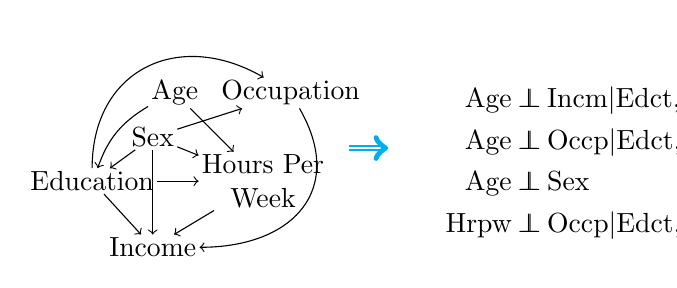
\begin{tikzpicture}
			\begin{scope}[xshift=-2.5cm, yshift=0.7cm, scale=0.7]
			\tikzstyle{every node}=[align=center, inner sep=1pt]
				\node (sex) at (-0.7, -0.8) {Sex};
				\node (age) at (-0.3, 0) {Age};
				\node (ed) at (-1.8, -1.6) {Education};
				\node (occ) at (1.8, 0) {Occupation};
				\node (hrpw) at (1.3, -1.6) {Hours Per \\ Week};
				\node (income) at (-0.7, -2.8) {Income};
			
				\draw[->]  (age) to[bend right=20] (ed);
				\draw[->]  (sex) to (ed);
				\draw[->]  (age) to (hrpw);
				\draw[->]  (ed) to (hrpw);
				\draw[->]  (sex) to (hrpw);
				\draw[->]  (ed) to (income);
				\draw[->]  (hrpw) to (income);
				\draw[->]  (occ) to[out=300, in=0, looseness=1.4] (income.east);
				\draw[->]  (sex) to (income);
				\draw[->]  (ed) to[out=90, in=150, looseness=1.3] (occ);
				\draw[->]  (sex) to (occ);	
			\end{scope}
			\begin{scope}[xshift=-3cm]
				\draw[thick, ->, double, cyan] (2.5,0) -- (3,0);
				\node[rectangle, align=center, inner sep=1pt] at (5, 0) {
					\begin{minipage}{.2\textwidth}
						\begin{equation*}
							\begin{split}
								\textnormal{Age} &\ci \textnormal{Incm} \rvert \textnormal{Edct, Hrpw, Sex} \\
								\textnormal{Age} &\ci \textnormal{Occp} \rvert \textnormal{Edct, Sex} \\
								\textnormal{Age} &\ci \textnormal{Sex} \\
								\textnormal{Hrpw} &\ci \textnormal{Occp} \rvert \textnormal{Edct, Sex} \\
							\end{split}
						\end{equation*}
					\end{minipage}
					};
			\end{scope}
		\end{tikzpicture}
		\caption{\todo[inline]{Show a full example of testing using this model}}
\end{figure}


\section{Background}
We represent uni-dimensional variables as $ X $ and multi-dimensional variables
as $ \bm{Z} $. We consider the case of estimating association between $ X $,
and $ Y $ is the presence of a set of conditioning variables $ \bm{Z} = Z_1,
\cdots, Z_k $, potentially being an empty set $ \bm{Z} = \emptyset $. We use $
\rvert \bm{Z} \rvert $ to denote the cardinality of the variable $ \bm{Z} $. We
consider various scenarios where the variables $ X $, $ Y $ and $ \bm{Z} $
could be either discrete, ordinal, or continuous. With mixed data, we mean an
arbitrary mix of variable types among $ X $, $ Y $, and $ \bm{Z} $.

We consider the problem of estimating the partial (or conditional) association
between $ X $ and $ Y $ in the presence of the conditioning set $ Z $. When $ Z
= \emptyset $, this is equivalent to the marginal association between $ X $ and
$ Y $.

\todo[inline]{Add more notation as they come}

\subsection{Measures of Association}
In this section, we give a background on some of the commonly used effect size
measures in the context of CI testing.

\paragraph{$ X $ and $ Y $ are continuous}
In the case when $ \bm{Z} = \emptyset $, and when both $ X $ and $ Y $ are
continuous variables, Pearson's correlation coefficient based test can be used
which also gives an effect size measure. The p-value computation requires the
data to be normally distributed but other statistics can be used such as
Spearman's rank correlation, or Kendall's Tau.

In the case when $ \bm{Z} \neq \emptyset $, then partial correlations can be used.
In this case we first compute the residuals of $ X $ and $ Y $ using $ \bm{Z} $ as 
the predictor. We start by training two model $ X \sim \bm{Z} $ and $ Y \sim \bm{Z} $.
Then the residuals are computed for both as $ R_X = X - \hat{X} $ and $ R_Y = Y - \hat{Y} $.
After this we can do a normal non-conditional test on $ R_X $ and $ R_Y $.

\paragraph{All variables are discrete}

When $ \bm{Z} = \emptyset $, in the case of discrete variables, chi-squared test can be used. Effect size 
measures such as Cram\'er's V are available for it.

When $ \bm{Z} \neq \emptyset $, we can do stratification.


\paragraph{$ X $ is ordinal and $ Y $ is continuous}
Polyserial Correlation

When $ \bm{Z} = \emptyset $, ordinal variable can be assumed to be coming from a thresholded normal distribution, estimate the thresholds and latent variable to compute 
the correlation coefficient.

\paragraph{$ X $ and $ Y $ are ordinal}
Polychoric Correlation

\paragraph{Mixed data}
Recently multiple tests for mixed data have been proposed but they do not have
an effect size measure. We propose one based on canonical correlations.

\subsection{Canonical Correlation}
Canonical correlations are generalization of correlations to multi-dimensional variables.

\begin{definition}
	Given two sets of random variables $ \bm{U} = (U_1, U_2, \cdots, U_p) $
	and $ \bm{V} = (V_1, V_2, \cdots, V_q) $, canonical correlation between
	them, $\rho(\bm{U}, \bm{V}) $ is defined as:
		
	\begin{equation}
		\rho(\bm{U}, \bm{V}) = \sup_{a, b} \frac{a^T \Sigma_{\bm{U}\bm{V}} b}{\sqrt{a^T \Sigma_{\bm{U}\bm{U}} a} \sqrt{b^T \Sigma_{\bm{V}\bm{V}} b}}
	\end{equation}

\end{definition}
	
	Canonical correlations try to find linear transformations $ a $ and $ b
	$ of $ \bm{U} $ and $ \bm{V} $ such that the correlations between the
	columns of $ a^T \bm{U} $ and $ b^T \bm{V} $ is maximized. The
	individual columns of $ a^T \bm{U} $ and $ b^T \bm{V} $ are
	independent. In the case when $ \rvert U \rvert = \rvert V \rvert = 1$,
	canonical correlations are equivalent to Pearson's correlation
	coefficient.

Multiple effect sizes measures based on canonical correlation are available.
\begin{itemize}
	\item Wilks' Lambda: $ \Lambda = \prod (1 - \phi_i^2) $
	\item Roy's Largest Root: $ \theta = \phi_{\max}^2 $
	\item Pillai's Trace: $ \tau = \sum \phi_i^2 $
\end{itemize}
We use Pillai's Trace in this paper. \todo[inline]{Why?}.

\section{Measure of Association for mixed data}
In this section, we use canonical correlations to define an effect size measure
for mixed data CI tests. Our approach is similar to the approach used for the
continuous variable case. 

\subsection{No conditional variables}
When we have no conditonal variables, we need to convert the variables into 

\subsection{Conditional Case}

\subsection{Connection to special cases}

\section{Web Tool}
As most of the DAGs in practice are built manually, we use our mixed data effect size measure to build a web-tool that aids researches in building DAGs.

% \begin{figure}
% 	\centering
% 	\begin{subfigure}{0.5\textwidth}
% 		\includegraphics[scale=0.25]{../../presentations/2024_05_das/2.png}
% 	\end{subfigure}%
% 	\begin{subfigure}{0.5\textwidth}
% 		\includegraphics[scale=0.25]{../../presentations/2024_05_das/5.png}
% 	\end{subfigure}
% 	\caption{Screenshots of the web-tool. \todo[inline]{Insert screenshots of the web-tool}}
% \end{figure}

\section{Empirical Analysis}
To compare how well does creating a graph manually based on effect sizes and
p-value compare to algorithmic approaches, we performed some empirical
analysis.

\subsection{Simulating an expert}
To simulate an expert building a model manually, we wrote a simple greedy simulation as shown in the Figure. The expert always starts with a graph with
no edges and chooses the pair of variables with the highest correlation between them. The expert based on some accuracy measure decides the direction
of the edge between these variables such that the new added edge does not create a cycle in the DAG.

\todo[inline]{Summarize this section and equation in an algorithm}
\todo[inline]{Show a consistency proof for this expert simulation}

\begin{equation}
	\begin{split}
		x &= \textnormal{rand}([0, 1]) \\
		O(\alpha) &= \begin{cases} 
			M \rightarrow Y, & \textnormal{if  } x <= \alpha \\
			\textnormal{rand}(M \rightarrow Y, M \leftarrow Y, None) & \textnormal{otherwise} \\
				\end{cases} \\
	\end{split}
\end{equation}

% \begin{algorithm}
% 	\caption{Expert Simulation}
% 	\While{True}{
% 	   $ e \gets \textnormal{Effects}(G) > \textnormal{THRESHOLD} $\;
% 	   $ e \gets e - \textnormal{blacklist} $\;
% 	   \If {$ e = 0 $}{
% 		$ G \gets G - e $ \;
% 		$ \textnormal{blacklist} \gets \textnormal{blacklist} \cup e $\;
% 	   } \;
% 	   \If{$ \textnormal{len}(e) = 0$}{
% 		   $ \textnormal{return}(G) $\;
% 	   }
% 	   $ X, Y \gets \max_{X, Y} e $\;
% 	   $ dir \gets Expert(X, Y, \alpha) $\;
% 	   $ G \gets G \cup dir $\;
% 	}
% 
% \end{algorithm}

After adding each edge, we also check if the p-value of any existing edge shows independence. If that happens we remove that edge and blacklist that edge. 
Blacklisted edges are not suggested to the expert in future iterations. We repeat this till we have explained all the correlations in the dataset.

There is a possibility that this greedy expert gets stuck at incorrect graph structures as it does not do any backtracking to fix its earlier mistakes.


\subsection{Results}
\begin{figure}
	\begin{subfigure}{0.5\textwidth}
		\includegraphics{../code/plots/shd_ribbon.pdf}
	\end{subfigure}
	\begin{subfigure}{0.5\textwidth}
		\includegraphics{../code/plots/sid_ribbon.pdf}
	\end{subfigure}
\end{figure}

\section{Conclusions}
\subsection{Using LLMs as experts}

\bibliography{references}
\end{document}
